\documentclass[11pt, oneside]{article} 
\usepackage{geometry}
\geometry{letterpaper} 
\usepackage{graphicx}
	
\usepackage{amssymb}
\usepackage{amsmath}
\usepackage{parskip}
\usepackage{color}
\usepackage{hyperref}

\graphicspath{{/Users/telliott_admin/Dropbox/Tex/png/}}
% \begin{center} 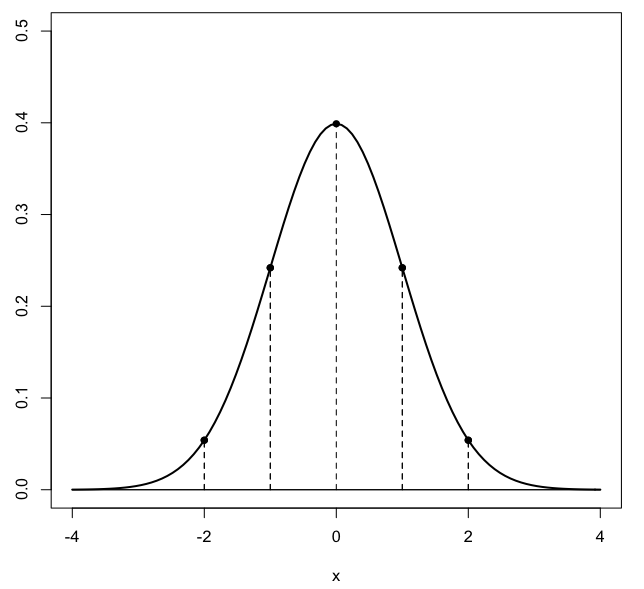
\includegraphics [scale=0.4] {gauss3.png} \end{center}

\title{Matrices}
\date{}

\begin{document}
\maketitle
\Large
So far we've only done one multiplication at a time.  Now we graduate to computing what are often called \textbf{dot products}.

Here's an example:
\begin{verbatim}
[2,3,1,1] * [2,1,1,3]
\end{verbatim}

The way this is done is to compute the product for each corresponding pair (i.e. $(2 * 2), (3 * 1), (1 * 1), (1 * 3)$) and then add them together by XOR.

\[ (2 * 2) \oplus (3 * 1) \oplus (1 * 1) \oplus (1 * 3) \]

In binary notation:

\begin{verbatim}
10 * 10 = 100
11 * 01 = 011
01 * 01 = 001
01 * 11 = 011
          ---
          101
\end{verbatim}
The answer is $101 = 5$.  It isn't hard to code something like:
\begin{verbatim}
def xor_reduce(L):
    r = 0
    for n in L:
        r = r ^ n
    return r

def dot(L1,L2):
    rL = [gm(x,y) for x,y in zip(L1,L2)]
    return xor_reduce(rL)
\end{verbatim}

The next idea is to put numbers into rows and columns (matrix format), like:
\[
\begin{matrix}
2 & 3 & 1 & 1 \\
1 & 2 & 3 & 1 \\
1 & 1 & 2 & 3 \\
3 & 1 & 1 & 2
\end{matrix}
\]

What can we do with this?  Try multiplying the matrix from above times a column (often called a vector):

\[
\begin{matrix}
2 & 3 & 1 & 1 \\
1 & 2 & 3 & 1 \\
1 & 1 & 2 & 3 \\
3 & 1 & 1 & 2
\end{matrix}
\ \ \times \ \ 
\begin{matrix}
2 \\
1 \\
1 \\
3 
\end{matrix}
\]

The result is also a vector, or a column, where the first (top) value is the dot product of the top row of the matrix with the elements of the column.  This is the same calculation as we carried out above, and the result is $5$.  Here is the whole thing:

\[
\begin{matrix}
2 & 3 & 1 & 1 \\
1 & 2 & 3 & 1 \\
1 & 1 & 2 & 3 \\
3 & 1 & 1 & 2
\end{matrix}
\ \ \times \ \ 
\begin{matrix}
2 \\
1 \\
1 \\
3 
\end{matrix}
\ \ = \ \ 
\begin{matrix}
5 \\
0 \\
4 \\
0 
\end{matrix}
\]

How did we get those zeros?  The computation for that zero (just below the $5$) is the \emph{second} row dotted with the column:
\[ 1,2,3,1 \times 2,1,1,3 = 1 * 2 \oplus 2 * 1 \oplus 1 * 3 \oplus 3 * 1 \]
We don't even have to calculate.  We obtain:
\[ 1 * 2 \oplus 2 * 1 = 0 \]
\[ 1 * 3 \oplus 3 * 1 = 0 \]

Duplicate computations always cancel.

It can be hard to keep track of which row we need at any one time.  The way I like to do this is to put the second multiplicand above the space where we're going to write the answer.

\[ \ \ \ \ \ \ \ \ \ \ \ \ \ \  \ \ \ \ \ 
\begin{matrix}
2 \\
1 \\
1 \\
3 
\end{matrix}
\]
times
\[
\begin{matrix}
2 & 3 & 1 & 1 \\
1 & 2 & 3 & 1 \\
1 & 1 & 2 & 3 \\
3 & 1 & 1 & 2
\end{matrix}
\ = \ \ \
\begin{matrix}
a_{11} \\
a_{21} \\
a_{31} \\
a_{41} 
\end{matrix}
\]

The subscript on $a_{21}$ means that value is the product of row $2$ and column $1$ (here there is only one column).

We can also multiply two matrices together.  If we label this matrix as \textbf{fM} (f for forward), try multiplying it times itself.

\pagebreak

\[ \ \ \ \ \ \ \ \ \ \ \ \ \ \  \ \ \ \ \
\begin{matrix}
2 & \ \  3 & \ \  1 & \ \  1 \\
1 & \ \  2 & \ \  3 & \  \ 1 \\
1 & \ \  1 & \ \  2 & \  \ 3 \\
3 & \ \  1 & \ \  1 & \  \ 2
\end{matrix}
\]
times
\[
\begin{matrix}
2 & 3 & 1 & 1 \\
1 & 2 & 3 & 1 \\
1 & 1 & 2 & 3 \\
3 & 1 & 1 & 2
\end{matrix}
\ = \ \ \
\begin{matrix}
a_{11} & a_{12} & a_{13} & a_{14} \\
a_{21} & a_{22} & a_{23} & a_{24} \\
a_{31} & a_{32} & a_{33} & a_{34} \\
a_{41} & a_{42} & a_{43} & a_{44}
\end{matrix}
\]

For example, $a_{21}$ is the dot product of the second row and the first column.

If this explanation doesn't make sense see wikipedia.  

\url{https://en.wikipedia.org/wiki/Matrix_multiplication}

Here are two figures I found on the web, one from that page:

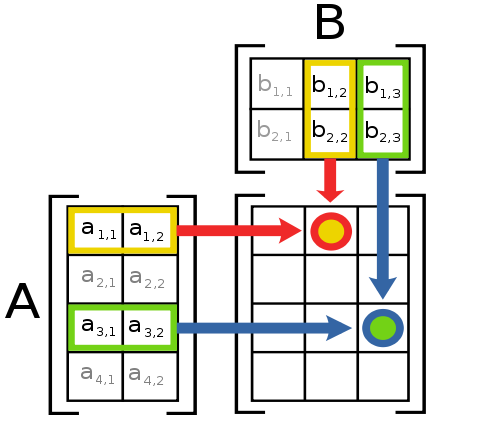
\includegraphics [scale=0.3] {mm1.png}
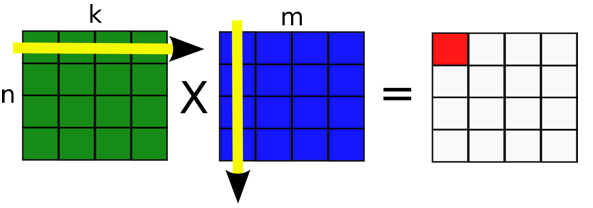
\includegraphics [scale=0.4] {mm2.png}

The vertical alignment is a pain to typeset, so I will just do this:
\[  
\begin{matrix}
2 & 3 & 1 & 1 \\
1 & 2 & 3 & 1 \\
1 & 1 & 2 & 3 \\
3 & 1 & 1 & 2
\end{matrix}
\ \times \ \
\begin{matrix}
2 & 3 & 1 & 1 \\
1 & 2 & 3 & 1 \\
1 & 1 & 2 & 3 \\
3 & 1 & 1 & 2
\end{matrix}
\ = \ \ 
\begin{matrix}
5 & 0 & 4 & 0 \\
0 & 5 & 0 & 4 \\
4 & 0 & 5 & 0 \\
0 & 4 & 0 & 5
\end{matrix}
\]

This is fairly tedious, since there are four multiplications and three XORs for each place in the table.

I won't show the code but I wrote a routine to do matrix multiplication with these matrices and format the results.  See

\url{https://github.com/telliott99/Crypto/blob/master/AES-math/README.md}

The matrix we obtained is sort of interesting.  Half the entries are zero, and the rows are shifted right as we go down.  But what is very interesting is what happens with one more multiplication:

\[  
\begin{matrix}
2 & 3 & 1 & 1 \\
1 & 2 & 3 & 1 \\
1 & 1 & 2 & 3 \\
3 & 1 & 1 & 2
\end{matrix}
\ \times \ \
\begin{matrix}
5 & 0 & 4 & 0 \\
0 & 5 & 0 & 4 \\
4 & 0 & 5 & 0 \\
0 & 4 & 0 & 5
\end{matrix}
\ = \ \ 
\begin{matrix}
14 & 11 & 13 & 9 \\
9 & 14 & 11& 13 \\
13 & 9 & 14 & 11 \\
11 & 13 & 9 & 14
\end{matrix}
\]

This matrix will be familiar if you've been looking at AES.  When encrypting by AES we use what I called the forward matrix \textbf{fM}.  The above matrix I called the reverse matrix \textbf{rM}.  We multiply by \textbf{rM} to reverse the \textbf{fM} step.

The reason it works is that
\[  
\begin{matrix}
2 & 3 & 1 & 1 \\
1 & 2 & 3 & 1 \\
1 & 1 & 2 & 3 \\
3 & 1 & 1 & 2
\end{matrix}
\ \times \ \
\begin{matrix}
14 & 11 & 13 & 9 \\
9 & 14 & 11 & 13 \\
13 & 9 & 14 & 11 \\
11 & 13 & 9 & 14
\end{matrix}
\ = \ \ 
\begin{matrix}
1 & 0 & 0 & 0 \\
0 & 1 & 0 & 0 \\
0 & 0 & 1 & 0 \\
0 & 0 & 0 & 1
\end{matrix}
\]

Commutativity is not generally true for matrices, but in \emph{this case} it is so:

\[  
\begin{matrix}
14 & 11 & 13 & 9 \\
9 & 14 & 11 & 13 \\
13 & 9 & 14 & 11 \\
11 & 13 & 9 & 14
\end{matrix}
\ \times \ \
\begin{matrix}
2 & 3 & 1 & 1 \\
1 & 2 & 3 & 1 \\
1 & 1 & 2 & 3 \\
3 & 1 & 1 & 2
\end{matrix}
\ = \ \ 
\begin{matrix}
1 & 0 & 0 & 0 \\
0 & 1 & 0 & 0 \\
0 & 0 & 1 & 0 \\
0 & 0 & 0 & 1
\end{matrix}
\]

The reason for commutativity is the repeated structure in the matrices.

Let's just do two of those dot products.  There is no irreducible polynomial needed because the numbers are so small.
\[ 14,11,13,9 \times 2,1,1,3 = 28, 11, 13, 27 \]
The XOR is
\begin{verbatim}
11100
01011
01101
11011
-----
00001
\end{verbatim}
and
\[ 9,14,11,13 \times 2,1,1,3 = 18,14, 11,39 \]
[ This has an error in the last figure ]

These are a bit tricky.  All results so far are equal to those from decimal multiplication, but the fourth is not.
\begin{verbatim}
 1101 = 13
   11 = 3
 ----
 1101
11010
-----
10111 = 23
\end{verbatim}
The crucial thing is that $10111 = 23$ is smaller than 32 so then the XOR is
\begin{verbatim}
10010 = 18
01110 = 14
01011 = 11
10111 = 23
------
00000
\end{verbatim}

If you look at the computations for each coefficient in the matrix, you'll see that the same computations are done for $\textbf{fM} \times \textbf{rM}$ as for $\textbf{rM} \times \textbf{fM}$.

So finally, we have that:

[\textbf{fM}]$^3$ = \textbf{fM} $\times$ \textbf{fM} $\times$ \textbf{fM} = \textbf{rM}

and

[\textbf{fM}]$^4$ = \textbf{rM} $\times$ \textbf{fM} = \textbf{I}

\textbf{I} is the identity matrix. \textbf{I} $\times$ any other matrix is equal to that matrix.  So if \textbf{P} is some matrix we're working on during encryption and we do 

\textbf{fM} $\times$ \textbf{P} = \textbf{C}

then

\textbf{rM} $\times$ (\textbf{fM} $\times$ \textbf{P})

= (\textbf{rM} $\times$ \textbf{fM}) $\times$ \textbf{P} = \textbf{I} $\times$ \textbf{P} = \textbf{P}



\end{document}